%% \chapter[htoc-titlei][hhead-titlei]{htitlei}
%% -----------------------------------------------------------------------------
\chapter[Alignment of the ATLAS Inner Detector][Alignment of the ATLAS Inner Detector]{Alignment of the ATLAS Inner Detector}
\label{ch:alignment}

As a charged particle passes through the ATLAS ID, it leaves \emph{hits} in the sensors along its path in the form of ionization.
The particle's trajectory, or \emph{track}, can be reconstructed from a fit to these hits via the procedure described in Section~\ref{detector:track_reconstruction}.
In order to reconstruct an accurate particle track, it is necessary to know where in space each hit occured as precisely as possible, which in turn requires knowledge of the physical location of the sensor that registered the hit.
If one of the sensors is displaced relative to its expected position in the known detector geometry, or \emph{misaligned}, the assumed location of the corresponding hit will not match its actual location, resulting in inaccurate track parameters and a poor track fit.
The first misalignments were a result of not knowing the exact positions of each sensor after the inital installation of the detector.
Subsequent misalignments occur when sensors shift due to mechanical stress and strain, which can be the result of cycles in ATLAS's magnetic field, changes in operating temperatures, or when components are removed and replaced during maintenance.
%These misalignments in the ID result in poor track reconstruction quality and ultimately degrade the overall detector resolution.
A visualization of how a misaligned detector element can affect the track reconstruction is shown in Figure~\ref{fig:alignment_effects_misalign}. %\TODO{ there has to be a better way to introduce this figure -- i haven't talked about residuals yet}

In order to correct the misalignments, the ID alignment procedure is applied to accurately determine the physical position and orientation of each detector element.
The baseline accuracy of the alignment is required to be such that the track parameter resolutions are not degraded by more than 20\% with respect to those derived from a perfect detector geometry\footnote{The so-called \emph{perfect geometry} refers to the description of the ATLAS detector in which every sensor precisely matches its design specifications.  The perfect geometry contains no misalignments, and the position of each sensor is known exactly.}~\cite{1997.id-tdr-1}.
This corresponds to a precision of better than $10~\mum$ in the positioning of the elements of the silicon detectors~\cite{2011.alignment-7tev}.

This chapter covers the ID alignment algorithm and procedure, its implementation during the 2015 data taking period, and the steps taken to measure momentum biases that may exist after alignment.  

\begin{figure}[htbp]
  \centering
  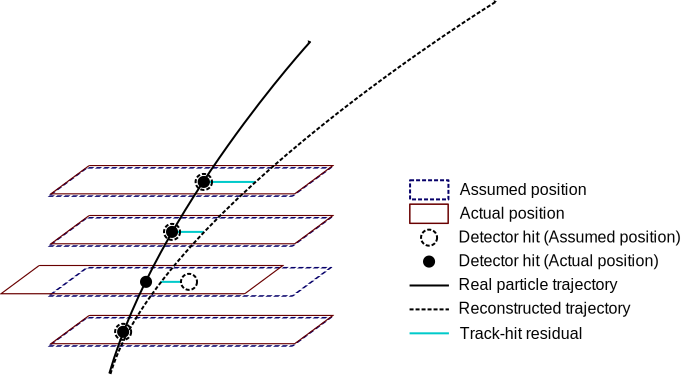
\includegraphics[width=.8\textwidth]{figs/alignment/misalignment}
  \caption{Graphical representation of the effect of a misaligned detector element.  The reconstructed particle track (dashed arrow) differs from the actual trajectory of the particle (solid arrow) due to a shift in the third detector element.  The cyan lines represent the track-to-hit residuals.}
  \label{fig:alignment_effects_misalign}
\end{figure}

%In order for the subdetectors of the ID to operate at their designed precisions, it is essential that the locations of the sensors be known as precisely as possible.
%Differences between the expected and actual positions of a sensor can result in displaced particle hits and degrade track reconstruction quality.
%These misalignments can occur for any number of reasons, including but not limited to elements shifting during maintenance periods or cycles in ATLAS's magnetic field, or simply small movements during normal detector operations.
%Since it is not practical to physically correct the positions of hundreds of thousands of detector elements to micron-level precision by hand, the alignment instead updates a database containing the best-known positions of each sensor.
%The effects of misalignments and the steps taken to correct and monitor them are detailed in this chapter.

%\section{Introduction to ID Alignment}\label{align:introduction}
%%% \chapter[htoc-titlei][hhead-titlei]{htitlei}
%% -----------------------------------------------------------------------------
\chapter[Introduction][Introduction]{Introduction}

% If you want space after a footnote, you need to force it like so.
The Standard Model (SM)\footnotemark~has been remarkably successful...
\footnotetext{Here's a footnote.}


\section{The alignment method}\label{align:method}
% define residuals
% alignment levels

The alignment procedure uses track-based algorithm that updates the locations of detector elements in order to minimize the set of track-hit \emph{residuals}.
These residuals are defined as the distance between the fitted track position in a given detector element to the position of the hit recorded by the same element.
Tracks in ATLAS are parameterized as five-dimensional vectors~\cite{2006.atlas-tracking-model}:%follow helical trajectories and are parameterized as five-dimensional vectors~\cite{2006.atlas-tracking-model}:
\begin{equation}
  \vec{\tau} = (d_0,z_0,\phi_0,\theta,q/p)
\end{equation}
where $d_0$ and $z_0$ are the transverse and longitudinal impact parameters with respect to the origin, respectively, $\phi_0$ is the azimuthal angle of the track at the point of closest approach to the origin, $\theta$ is the polar angle, and $q/p$ is the charge of the track divided by its momentum.
The residual for the $i^{\textrm{th}}$ hit of a given track can then be written in terms of the track parameters $\vec{\tau}$ and the alignment parameters $\vec{a}$ that describe the hit location~\cite{2005.global-chi2-alignment}:
\begin{equation}
  r_i(\vec{\tau},\vec{a}) = (\vec{m}_i - \vec{e}_i (\vec{\tau},\vec{a}))\cdot\hat{k}
\end{equation}
where $\vec{e}_i$ is the intersection point of the extrapolated track with the sensor, $\vec{m}_i$ is the position of the associated hit within the sensor, and $\hat{k}$ is the unit vector defining the direction of the measurement within the sensor.
$\vec{r}$ is then the vector of residuals for the given track.
The effect of a misaligned detector element on the track reconstruction and the resulting track-hit residuals is shown in Figure~\ref{fig:alignment_effects_misalign}. \TODO{ there has to be a better way to introduce this figure}

\begin{figure}[htbp]
  \centering
  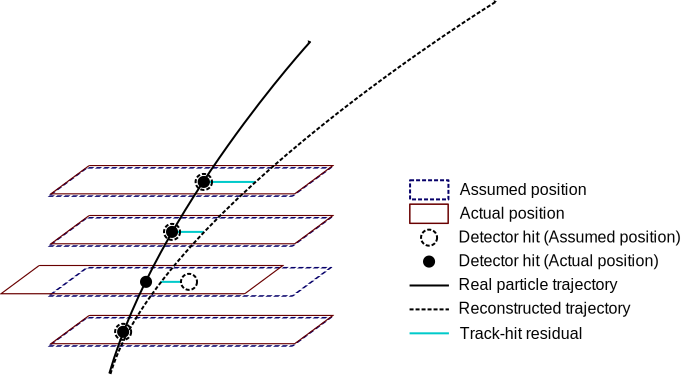
\includegraphics[width=.8\textwidth]{figs/alignment/misalignment}
  \caption{Graphical representation of the effect of a misaligned detector element.  The reconstructed particle track (dashed arrow) differs from the actual trajectory of the particle (solid arrow) due to the shift in one of the detector elements.  The cyan lines represent the track-to-hit residuals.}
  \label{fig:alignment_effects_misalign}
\end{figure}

% the alignment constants are those that minimize the track-hit residuals
A $\chi^2$ function can be built from the residuals of all collected tracks:
\begin{equation}
  \chi^2 = \sum\limits_{\textrm{tracks}}\vec{r}^{T}V^{-1}\vec{r}
  \label{eq:alignment_chi2}
\end{equation}
where $V$ is the covariance matrix of the hit measurements.
The $\chi^2$ function is then minimized with respect to the alignment parameters $\vec{a}$, which contain all degrees of freedom being aligned.
The minimzation condition with respect to $\vec{a}$ is:
\begin{equation}
  \frac{d\chi^2}{d\vec{a}} = 0 ~~ \rightarrow ~~ 2\sum\limits_{\textrm{tracks}}\bigg(\deriv{\vec{r}}{\vec{a}}\bigg)^{T}V^{-1}\vec{r} = 0
  \label{eq:alignment_chi2_min_condition}
\end{equation}
This equation can be difficult to solve exactly, so the residual is rewritten as a first order Taylor expansion:
\begin{equation}
  %\vec{r} = \vec{r}_0+\frac{\partial\vec{r}}{\partial\vec{\tau}}\delta\vec{\tau}+\frac{\partial\vec{r}}{\partial\vec{a}}\delta\vec{a}
  \vec{r} = \vec{r}_0+\deriv{\vec{r}}{\vec{a}}\delta\vec{a}
  \label{eq:alignment_residual_taylor}
\end{equation}
where $\vec{r}_0$ is dependent on an initial set of track and alignment parameters $\vec{\tau}_0$ and $\vec{a}_0$, respectively; the track parameter dependence has also been folded into the total derivative $\deriv{\vec{r}}{\vec{a}}$.
Equation~\ref{eq:alignment_residual_taylor} can then be inserted into the minimization condition from Equation~\ref{eq:alignment_chi2_min_condition} to give:
\begin{equation}
  \Bigg[ \sum\limits_{\textrm{tracks}}\bigg(\deriv{\vec{r}}{\vec{a}}\bigg)^{T}V^{-1}\deriv{\vec{r}}{\vec{a}} \Bigg]\delta\vec{a} + \sum\limits_{\textrm{tracks}}\bigg(\deriv{\vec{r}}{\vec{a}}\bigg)^{T}V^{-1}\vec{r}_0 = 0
  \label{eq:alignment_chi2_min_taylor}
\end{equation}
From this equation, the alignment matrix $\mathcal{M}_a$ and alignment vector $\vec{\nu}_a$ can be defined:
\begin{equation}
  \mathcal{M}_a = \sum\limits_{\textrm{tracks}}\bigg(\deriv{\vec{r}}{\vec{a}}\bigg)^{T}V^{-1}\deriv{\vec{r}}{\vec{a}}
  \label{eq:alignment_matrix}
\end{equation}
\begin{equation}
  \vec{\nu}_a = \sum\limits_{\textrm{tracks}}\bigg(\deriv{\vec{r}}{\vec{a}}\bigg)^{T}V^{-1}\vec{r}_0
  \label{eq:alignment_vector}
\end{equation}
Finally, the alignment corrections $\delta\vec{a}$ can be solved for by inverting the alignment matrix:
\begin{equation}
  \delta\vec{a} = -\mathcal{M}_a^{-1}\vec{\nu}_a
  \label{eq:alignment_corrections}
\end{equation}
%The \emph{alignment constants} are the values of $\vec{a}$ that minimize the track-hit residuals.
which is a linear system of equations with a number of equations equal to the number of alignment degrees of freedom.


\TODO{In practice, the alignment algorithm is iterative . . .}
\TODO{make figure showing iterative procedure as in PoS}

\subsection{Alignment levels}\label{align:levels}


\section{Early 2015 alignment of the ATLAS detector}\label{align:2015}
At the end of Run 1, the LHC was shut down for upgrades and maintenance.
During this time, a number of upgrades were performed on the ATLAS detector, including the installation of a new innermost layer of the Pixel detector, the Insertable B-Layer (IBL)~\cite{2010.ibl-tdr}. \TODO{This will certainly be defined in the detector description, so maybe the citation and abbreviation are not needed}
These changes to the ID required some detector components to be removed temporarily, and many elements shifted relative to each other over the course of the maintenance process.
In order to correct for these large detector movements prior to \com{13} collision data taking, an alignment was performed using cosmic ray data collected in early 2015~\cite{2015.alignment-2015-cosmic}.
This alignment was able to correct for the majority of the large detector-wide misalignments as well as determine the global position of the IBL at the micron level.
%Due to the relatively low statistics available in the cosmic ray data, the alignment was performed up to L3 in the Pixel barrel and IBL and only up to L2 in the SCT (barrel and end-caps) and the Pixel end-caps; the TRT was kept fixed as a reference point.

In June of 2015, shortly after the data taking period began, the first track-based alignment of the refurbished ID was performed using $\mathcal{L} = 7.9~\mathrm{pb}^{-1}$ of \com{13} $pp$ collision data~\cite{2015.alignment-13tev}.
Starting from the initial geometry determined by the cosmic ray alignment, referred to hereafter as the \emph{March alignment}, an improved set of alignment constants, called the \emph{June alignment}, was derived from a data set of approximately 1.4 million selected tracks.
For comparison, a MC sample containing approximately 2.7 million tracks was constructed from dijet events simulated using a perfect detector geometry; the MC events are reweighted to match the $\eta$ and $\pt$ distributions found in the data.
Additional validation of the alignment results uses a set of cosmic ray data collected by the detector during the LHC collisions.
\TODO{find some way of saying that this section follows the alignment note~\cite{2015.alignment-13tev}? or is it ok not to...}

\subsection{June alignment procedure}
The data set used as the input for the alignment contains a subset of physics events used for prompt reconstruction recorded at a rate of 10~Hz.
To ensure that only high quality tracks are used for the alignment, each track is required to have transverse momentum $\pt > 3\gev$, contain at least one hit in the Pixel detector, at least seven hits in the combined silicon detectors, and at least 25 hits in the TRT.

A full L3 alignment of the IBL was included in the March alignment; however, the IBL was operated at a temperature of $-20^{\circ}\textrm{C}$ during the cosmic data taking and at $-10^{\circ}\textrm{C}$ for collision data taking.
This proved to be significant, as it was observed that the IBL staves experience a temperature-dependent parabolic bowing in the local $x'$-direction of approximately $-10\mum/\textrm{K}$~\cite{2015.alignment-ibl-stability}.
As a result, a new L3 alignment of the IBL was essential in order to correct for the bowing.
Due to it being a brand new element of the detector as well as its importance in vertexing and $b$ jet tagging, aligning the IBL sensors with a high degree of precision was of great importance.

The June alignment was performed in two stages.
The first pass focused on any relative movements of the big structures.
The March alignment corrected for these as well; however, it was observed during Run 1 that these sort of misalignments are introduced by changing conditions in the detector~\cite{2014.alignment-performance-8tev}, such as in the cooling system or magnet power cycling, which may have occurred between the early cosmic data taking and the first \com{13} collisions.
The TRT detector was kept fixed for the entire first pass to act as a global reference frame.
The full alignment chain for the first pass consisted of the following steps:
%\begin{table}[htbp]
%  \centering
%  \begin{tabular}{l | l | l}
%    Step & Subdetector & Specific alignment \\ 
%    \hline\hline
%    \multirow{5}{*}{1} & IBL & Aligned at L1 \\
%    \cline{2-3}
%                      & \multirow{2}{*}{Pixel} & Barrel aligned at L1 \\
%                      &                        & End-caps aligned at L1 \\
%    \cline{2-3}
%                      & \multirow{2}{*}{SCT} & Barrel and end-caps aligned at L1 (fixed in $T_z$)\\%\footnote{The SCT barrel is fixed in $T_z$ in order to constrain global displacements along the $z$-axis, since the TRT is not sensitive in this direction} \\
%                      &                      & End-caps aligned at L1 \\
%    \hline
%    \multirow{5}{*}{2} & IBL & Aligned at L2 \\
%    \cline{2-3}       & \multirow{2}{*}{Pixel} & Barrel aligned at L2 \\
%                      &                        & End-caps aligned at L2 \\
%    \cline{2-3}       & \multirow{2}{*}{SCT} & Barrel and end-caps aligned at L2 \\
%                      &                      & End-caps aligned at L1 \\
%    \hline
%    \multirow{5}{*}{3} & IBL & Aligned at L27 \\
%    \cline{2-3}       & \multirow{2}{*}{Pixel} & Barrel aligned at L27 \\
%                      &                        & End-caps aligned at L27 ($T_x$, $T_y$, and $R_z$ only) \\
%    \cline{2-3}       & \multirow{2}{*}{SCT} & Barrel and end-caps aligned at L2 \\
%                      &                      & End-caps aligned at L1 \\
%    \hline
%    4 & IBL & Aligned at L3 \\
%    \hline
%  \end{tabular}
%  \caption{}
%  \label{tab:align_2015_first_pass}
%\end{table}
\begin{enumerate}
\item The IBL, Pixel, and SCT detectors were aligned at L1.  The SCT barrel was not aligned in $T_z$ in order to constrain global displacements along the $z$-axis, as the TRT is not sensitive to that degree of freedom.
\item The IBL, and Pixel barrel and end-caps, and SCT barrel were aligned at L2.  The SCT end-caps were aligned at L1.
\item The IBL and pixel barrel were aligned at L27, using all six degrees of freedom.  The Pixel end-cap disks were only aligned in the plane ($T_x$, $T_y$, and $R_z$).  The SCT was treated the same as in the previous step.
\item The IBL was aligned at L3 using all six degrees of freedom for each module.
\end{enumerate}

The second pass was performed with the goal of improving the resolution on the transverse impact parameter of the tracks.
This step includes an added constraint, where an impact parameter with respect to the beam spot is added to the track as a pseudo-measurement.
When the alignment algorithm minimizes the $\chi^2$, it will take care of the impact parameter minimization as well.
Once again, the TRT was kept fixed.
The stages of the second pass are listed below:
\begin{enumerate}
\item The IBL and Pixel detectors were aligned at L2 with the SCT fixed.
\item The IBL was aligned at L27
\item The IBL and Pixel barrel and end-caps were aligned at L3.
\end{enumerate}
The set of alignment constants obtained at the end of the second pass represents the June alignment.
The highest level of alignment over the course of the two passes for each subdetector is listed in Table~\ref{tab:align_june_levels}.

\begin{table}[htbp]
  \centering
  \begin{tabular}{l l | l}
    Detector & & Highest level of alignment\\
    \hline\hline
    IBL && L3 \\
    \hline
    \multirow{2}{*}{Pixel} & Barrel & L3 \\
                           & End-caps & L3 ($T_x$, $T_y$, and $R_z$ only) \\
    \hline
    \multirow{2}{*}{SCT} & Barrel & L2 (except $T_z$) \\
                           & End-caps & L1 \\
    \hline
    TRT && None\\
    \hline
  \end{tabular}
  \caption{Summary of the highest level of alignment applied to each ID subsystem when deriving the June alignment.}
  \label{tab:align_june_levels}
\end{table}

\subsection{Alignment results}
The primary measure of alignment quality is assessed by looking at the track-hit residual distributions.
A well-aligned subdetector will have gaussian-distributed residuals centered at zero with a width approximating the detector's resolution.
The residual distributions are constructed from the same selection of tracks that were used to perform the alignment, and are the focus of Section~\ref{align:2015_results_residual}.
A second check on the alignment involves observables sensitive to the track parameter resolution.
In this case, cosmic rays are used, making use of a ``split track'' technique that takes advantage of the top-to-bottom cosmic ray trajectory (compared to the center-out trajectory of collision tracks).
These checks are detailed in Section~\ref{align:2015_results_cosmic}

\subsubsection{Residual distributions from collisions}\label{align:2015_results_residual}
As mentioned previously, the primary focus of the June alignment campaign was on the IBL and the Pixel detectors.
The detectors are the closest to the beam line and have the finest resolutions of the ID subdetectors.
The residual distributions in local $x$ and $y$ of the IBL planar sensors\footnote{The IBL contains 12 planar sensors in the center of a stave, with four 3D sensors on either end.  Only the planar sensors are shown here due to low statistics in the 3D sensors as well as poor MC modeling of these sensors.} are shown in Figure~\ref{fig:align_2015_results_ibl}.
These and subsequent figures in this section compare the June and March alignments to the perfectly-aligned MC simulation.
Noticeable improvement in the distribution widths can be seen in both the local $x$- and $y$-directions, nearly matching the simulation in local $x$, which is the most sensitive direction.

Due to the temperature-dependent bowing of the IBL, it is also interesting to look at the means of the residual distributions for each ring of IBL sensors along the beam line, as shown in Figure~\ref{fig:align_2015_results_ibl_z}.
A deformation is clearly visible in the March alignment in both measurement directions, and the shape in the local $x$-direction is consistent with an average stave bowing due to the different operating temperature of the IBL during the March alignment and the $13\tev$ collisions.
This feature was nearly eliminated in both directions through the L3 alignment of the IBL sensors.

The local $x$ and $y$ residual distributions for the Pixel detector barrel and end-caps are shown in Figure~\ref{fig:align_2015_results_pix}.
The IBL is not included in the plots of the barrel.
Once again, the June alignment outperforms the March alignment and rivals the simulation in all but the barrel local $y$ residuals, likely indicating that further refinement in the local $y$ alignment of the IBL was needed.

\begin{figure}[htbp]
  \includegraphics[width=.48\textwidth]{figs/alignment/align2015/PIXIBL_Planar_xRES}
  \includegraphics[width=.48\textwidth]{figs/alignment/align2015/PIXIBL_Planar_yRES}
  \caption{Local $x$ (left) and local $y$ (right) residual distributions of the IBL planar sensors using the \com{13} collision data sample reconstructed using the June (black) and March (green) alignments.  The data is compared to a MC simulation using a perfect detector geometry (red).  The distributions are normalized to the same number of entries.}
  \label{fig:align_2015_results_ibl}.
\end{figure}

\begin{figure}[htbp]
  \includegraphics[width=.48\textwidth]{figs/alignment/align2015/IBL_xRESvsZ}
  \includegraphics[width=.48\textwidth]{figs/alignment/align2015/IBL_yRESvsZ}
  \caption{The mean of the local $x$ (left) and local $y$ (right) residual distributions as a function of the global $z$ position of each IBL module using the \com{13} collision data sample reconstructed using the June (black) and March (green) alignments.  The data is compared to a MC simulation using a perfect detector geometry (red).}
  \label{fig:align_2015_results_ibl_z}.
\end{figure}

\begin{figure}[htbp]
  \includegraphics[width=.48\textwidth]{figs/alignment/align2015/OLDPIXX}
  \includegraphics[width=.48\textwidth]{figs/alignment/align2015/PIXECX}\\
  \includegraphics[width=.48\textwidth]{figs/alignment/align2015/OLDPIXY}
  \includegraphics[width=.48\textwidth]{figs/alignment/align2015/PIXECY}
  \caption{Local $x$ (top) and local $y$ (bottom) residual distributions for the Pixel barrel (excluding the IBL, left) and end-caps (right) using the \com{13} collision data sample reconstructed using the June (black) and March (green) alignments.  The data is compared to a MC simulation using a perfect detector geometry (red).  The distributions are normalized to the same number of entries.}
  \label{fig:align_2015_results_pix}.
\end{figure}

Similar distributions for the SCT and TRT barrel and end-caps are shown in Figures~\ref{fig:align_2015_results_sct} and \ref{fig:align_2015_results_trt}, respectively.
Even though the TRT was not aligned at all, there is still some improvement in the width of the residuals between the March and June alignments due to the alignment of the other subdetectors improving the quality of the track fit.
The overall alignment of both these subdetectors despite neither being aligned at module-level indicates that the previous L3 alignment performed in Run 1 has not degraded significantly during the upgrade and maintenance period.

\begin{figure}[htbp]
  \includegraphics[width=.48\textwidth]{figs/alignment/align2015/SCTX}
  \includegraphics[width=.48\textwidth]{figs/alignment/align2015/SCTECX}
  \caption{Local $x$ residual distributions for the SCT barrel (left) and end-caps (right) using the \com{13} collision data sample reconstructed using the June (black) and March (green) alignments.  The data is compared to a MC simulation using a perfect detector geometry (red).  The distributions are normalized to the same number of entries.}
  \label{fig:align_2015_results_sct}.
\end{figure}

\begin{figure}[htbp]
  \includegraphics[width=.48\textwidth]{figs/alignment/align2015/TRTR}
  \includegraphics[width=.48\textwidth]{figs/alignment/align2015/TRTEC}
  \caption{Residual distributions for the TRT barrel (left) and end-caps (right) using the \com{13} collision data sample reconstructed using the June (black) and March (green) alignments.  The data is compared to a MC simulation using a perfect detector geometry (red).  The distributions are normalized to the same number of entries.}
  \label{fig:align_2015_results_trt}.
\end{figure}

\subsubsection{Track parameter resolution from cosmic rays}\label{align:2015_results_cosmic}

%\section{Additional alignment efforts}
%\subsection{L2 alignment of the TRT}
%\subsection{Alignment of the IBL}\label{align:ibl}
%thinking this should probably be a section not a subsection since it's not directly related to the 2015 paper i'm basing the previous section on... idk.


\section{Level 2 alignment of the TRT}\label{align:trt}
During validation of the final end-of-year reprocessing of the 2015 data, a misalignment was found in the barrel of the TRT detector, as several modules (triangular clusters of straws) showed rotations in the local $y$ coordinate.
The then-best available constants included a full L3 alignment of the silicon detectors and a separate L2 alignment of the TRT.
However, not all degrees of freedom were enabled when the TRT was aligned.
To correct for these tilts, an additional four iterations of L2 alignment was performed on the TRT enabling all available degrees of freedom ($T_x$, $T_y$, $R_x$, $R_y$, and $R_z$ in the barrel, and $T_x$, $T_y$, and $R_z$ for the endcaps).
Plots of the residual means from TRT barrel $\phi$-sectors containing modules affected by the tilt misalignment are shown in Figure~\ref{fig:align_trt_l2} before and after the L2 alignment.

\begin{figure}[htbp]
  \centering
  \includegraphics[width=.48\textwidth]{figs/alignment/trt/TRT_aveResVsStrawLayerModule0}
  \includegraphics[width=.48\textwidth]{figs/alignment/trt/TRT_aveResVsStrawLayerModule16}
  \caption{Residual means by straw layer in two TRT $\phi$-sectors affected by a tilt misalignment.  The tilts in each of the three modules are clearly visible in the red points representing the reconstructed data prior to alignment.  After four iterations of L2 alignment, the residual means in the gray points are flat.}
  \label{fig:align_trt_l2}
\end{figure}

Following the L2 alignment, some additional time was taken to determine if a full wire-by-wire L3 alignment of the TRT was necessary.
The TRT was last aligned at L3 during Run 1, but initial alignment campaigns in Run 2 did not show signs of misalignment (see, for example, the residual distributions shown earlier in Figure~\ref{fig:align_2015_results_trt}).
In order to assess the alignment more carefully, two dimensional residual maps in $\phi$ and $z$ were constructed for each layer in the TRT barrel and endcaps using the current alignment.
These maps were compared to a similar set using the L3 alignment from 2010, from which it was determined that the straw-level alignment indeed hadn't degraded, and a new L3 alignment was not needed.
The maps for the first layer of the TRT barrel are shown in Figure~\ref{fig:align_trt_map} for both sets of alignment constants.


\begin{figure}[htbp]
  \centering
  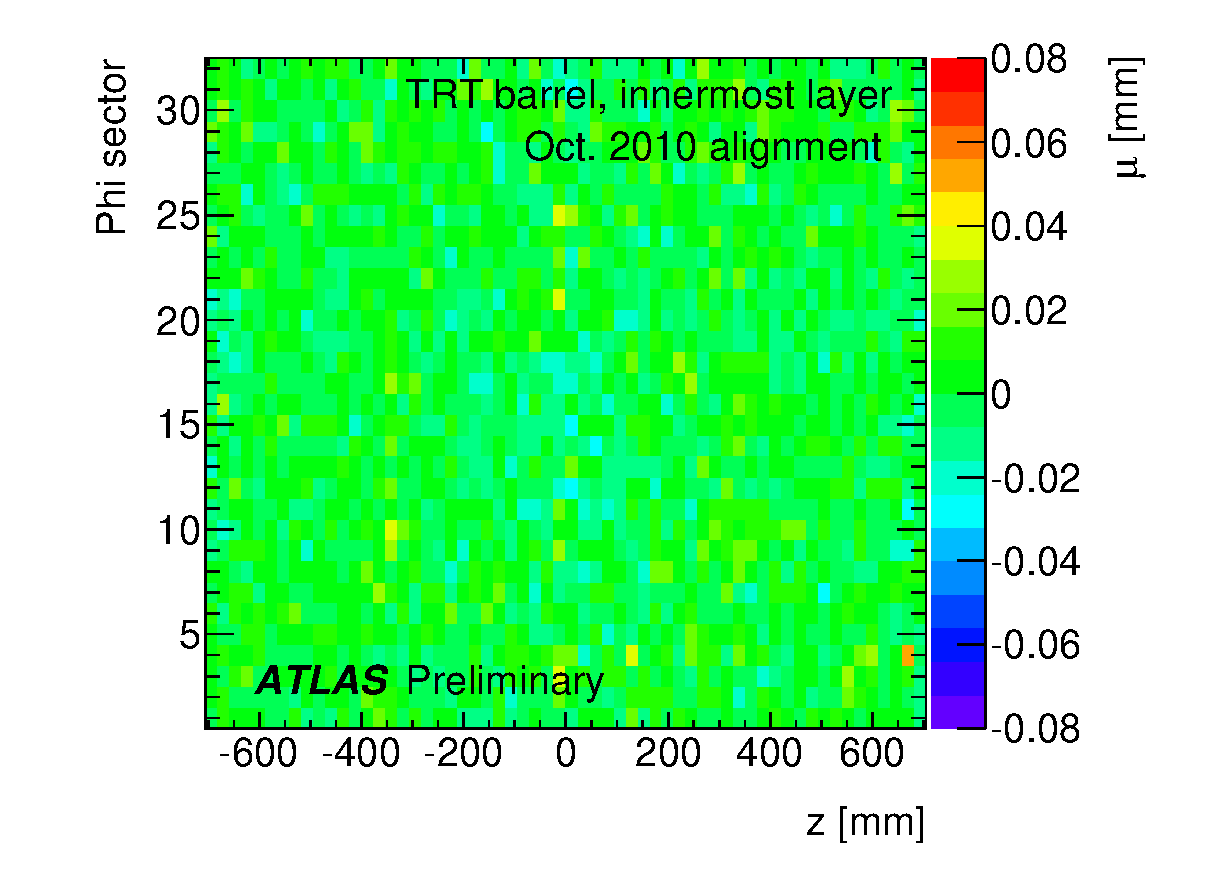
\includegraphics[height=.25\textheight]{figs/alignment/trt/TRT_barrel_ResMaps_Oct10}
  \includegraphics[height=.25\textheight]{figs/alignment/trt/trt_b_aveResVsPhiZ_l0_compare}
  \caption[Two dimensional map of residuals in the first layer of the TRT barrel vs $z$ and $\phi$.  Each bin represents the mean of a Gaussian fit to the TRT residuals in that bin.  The map on the left is after the L3 (wire-by-wire) alignment of the TRT performed in 2010, and the map on the right is after the L2 alignment at the end of 2015.  The $z$-axis for both plots use the same scale.]{Two dimensional map of residuals in the first layer of the TRT barrel vs $z$ and $\phi$.  Each bin represents the mean of a Gaussian fit to the TRT residuals in that bin.  The map on the left is after the L3 (wire-by-wire) alignment of the TRT performed in 2010, and the map on the right is after the L2 alignment at the end of 2015.  The $z$-axis for both plots use the same scale.  Left figure taken from~\cite{2011.alignment-7tev}.}
  \label{fig:align_trt_map}
\end{figure}


%\section{Alignment of the IBL}\label{align:ibl} % does this need a dedicated section? Perhaps a subsection of alignment method
%\input{sections/alignment/ibl_distortion.tex}

\section{Momentum bias from sagitta deformations}\label{align:bias}
A variety of weak mode deformations can exist in the detector even after alignment.
As mentioned previously, these weak modes consist of misalignments which don't affect the $\chi^2$ of the residuals and thus are not handled by the basic alignment algorithm.
In the presence of a weak mode, the description of the detector geometry can still provide efficient and high quality track fits, but there may also be systematic biases in one or more track parameters.
Several weak modes, their impacts on the reconstruction, and the steps taken to eliminate them are detailed in~\cite{2014.alignment-performance-8tev, 2012.alignment-systematics}. 
This section focuses specifically on sagitta distortions that result in a bias in the reconstructed track momentum.

These \emph{sagitta} distortions consist of detector movements orthogonal to the trajectory of the outgoing particle.
The effect on the reconstructed track curvature is different for positvely and negatively charged particles, resulting in a charge-antisymmetric bias.
This effect is illustrated in the curl deformation shown in Figure~\ref{fig:align_radial_distortion}.

In the plane transverse to ATLAS's magnetic field, outgoing particle tracks form circular arcs.
The sagitta is defined as the distance from the center of this arc to the center of its base, as shown in Figure~\ref{fig:align_sagitta}, and it represents the ``amount of bending'' in the track.
In the case where the sagitta $s$ is considerably smaller than the detector radius $R_0$, which is a valid assumption when working with high momentum tracks, the transverse momentum of a particle of charge $q$ can be written as~\cite{2018.alignment-radial-distortions}:
\begin{equation}
  \pt \propto q B \frac{R_0^2}{8s}
  \label{eq:align_pt_sagitta}
\end{equation}
where $B$ is the strengh of the detector's magnetic field.
If a sagitta bias is present, the track's transverse momentum shifts by~\cite{2012.alignment-systematics}:
\begin{equation}
  q/\pt\rightarrow q/\pt+\delta_s ~~~~~\textrm{or}~~~~~ \pt\rightarrow \pt\cdot(1+q\pt\delta_s)^{-1}
  \label{eq:align_pt_sagitta_bias}
\end{equation}
where $\delta_s$ is a universal bias parameter that uniquely defines the deformation.
Finally, since the reconstructed polar angle does not change under a sagitta deformation, the longitudinal component of the momentum scales along with the transverse component, and an equivalent equation can be written for the total momentum:
\begin{equation}
  p\rightarrow p\cdot(1+q\pt\delta_s)^{-1}
  \label{eq:align_p_sagitta_bias}
\end{equation}

\begin{figure}[htbp]
  \centering
  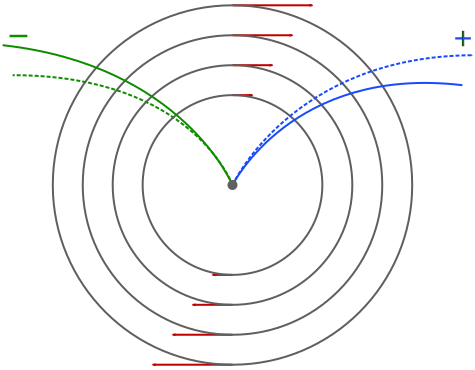
\includegraphics[width=.45\textwidth]{figs/alignment/radial-distortion}
  \caption{Representation of a curl distortion in the detector.  The image shows a cutaway in the transverse plane.  The deformation is represented by the red arrows, and the impact on the reconstructed positive (blue) and negative (green) tracks are shown.  The dashed lines represent the true particle trajectories, and the solid lines represent the reconstructed trajectories.}
  \label{fig:align_radial_distortion}
\end{figure}

\begin{figure}[htbp]
  \centering
  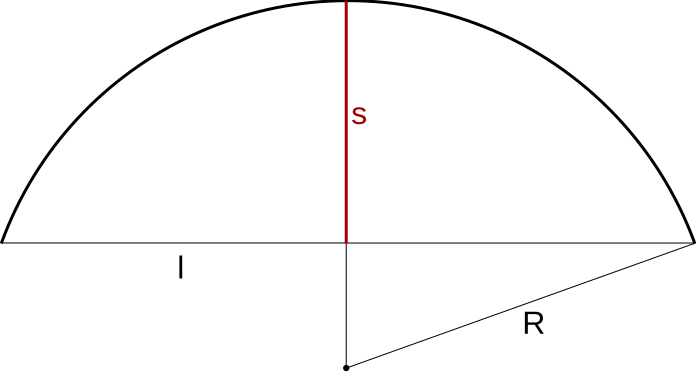
\includegraphics[width=.4\textwidth]{figs/alignment/sagitta}
  \caption{Geometric definition of the sagitta $s$ in relation to the length of the chord $l$ and the radius $r$ of a circular arc.}
  \label{fig:align_sagitta}
\end{figure}

\subsection{Sagitta bias monitoring with electron $E/p$}\label{align:eop}
Since a sagitta bias results in changes in the momentum of particles' tracks as measured by the ID, they can be identified using independent measurements from other systems in the detector.
One such method involves using the energy-momentum ratio of electrons ($E/p$).
Since the electron's energy is measured in ATLAS's calorimeter systems, it is not sensitive to any sagitta bias that may exist in the ID and the corresponding track momentum.
Under the assumption that the calorimeter response is independent of the charge of incoming particles, a charge-dependent momentum bias in the ID will manifest as a difference in the $E/p$ ratio for electrons and positrons.%\footnote{For the remainder of this section, electrons and positrons will collectively be referred to as ``electrons'' unless explicitly noted.}.

In the presence of a sagitta bias, the momentum will change according to Equation~\ref{eq:align_p_sagitta_bias} and the average measured $\eop$ can be written as:
\begin{equation}
  \eop^{\pm}\rightarrow\eop^{\pm}\pm\langle\et\rangle\delta_s
\end{equation}
where the approximation $\pt\approx\et$ is used.
Assuming that $\eop^+ = \eop^-$ in the absense of a bias, the sagitta bias parameter can be written as:
\begin{equation}
  \delta_s = \frac{\eop^+ - \eop^-}{2\langle\et\rangle}
\label{eq:align_eop_sagitta}
\end{equation}
If the kinematic selections for electrons and positrons are identical, the energy scale of the calorimeter will not factor into the $\eop$ difference; however, it will affect $\langle\et\rangle$ which would scale the measured $\delta_s$.
This is expected to be a small effect, as the energy scale for electrons has been measured at \com{13} with uncertainties on the per-mil level across the entire detector~\cite{2016.electron-photon-calibration}.

\subsubsection{Measuring $\eop$}
The $E/p$ ratio is measured using electrons and positrons from $\Zee$ events in order to obtain a high purity sample of electron candidates.
They are required to pass a basic selection criteria to ensure they are well measured by both the ID and the calorimeters:
\begin{itemize}
  \item $\et > 25~\gev$
  \item $|\eta| < 2.47$, excluding the calorimeter's barrel-to-endcap transition region in $1.37<|\eta|<1.52$
  \item Pass \tt{MediumLH} identification working point detailed in Section~\ref{detector:electron_reconstruction}
  \item Pass a selection of quality cuts, including a requirement that the electron be identified using cluster information in the calorimeter %author == 1 is cluster based only, author == 3 is cluster and track-based
  \item The associated track must have at least one hit in the IBL, three in the Pixel detector, and five in the SCT detector.
\end{itemize}
Events with exactly two opposite-charge electrons passing this selection with a dielectron invariant mass within $30~\gev$ of the $Z$ boson mass are then used for the $E/p$ calculation.

Since the size of the sagitta bias $\delta_s$ is not expected to be constant across the entire detector, a two-dimensional rectangular grid binned in detector $\eta$ and $\phi$ is constructed.
From the selected events, separate distributions of $E/p$ are made for electrons and positrons lying in each bin.
Each distribution is fit with Crystal Ball function\footnote{The Crystal Ball function is a proability density function consisting of a Gaussian core and a power-law tail.}, and the peak of the distribution is taken as the value of $\eop$.
If there is no bias on the track momentum in the bin, the peaks for electrons and positrons should match.
Example $E/p$ distributions including the Crystal Ball fits are shown in Figure~\ref{fig:alignment_eop_fit}.

It is important to emphasize that deviations from one in the \emph{ratio} of $\eop$ for electrons and positrons indicates that a momentum bias may be present.
The value of $\eop$ itself is not expected to equal one exactly, as the track momentum on average tends to be slightly lower than the energy measurement in the calorimeter.
This is due to the fact that if the electron were to radiate a photon, its momentum would change slightly, while it is likely that both the electron and the emitted photon would leave energy deposits near each other in the calorimeter and be reconstructed into the same object. 

\begin{figure}[htbp]
  \centering
  \includegraphics[width=.48\textwidth]{figs/alignment/eop/eop_fit_nobias}
  \includegraphics[width=.48\textwidth]{figs/alignment/eop/eop_fit_bias}
  \caption{$E/p$ distributions of electrons and positrons in two different $\eta$-$\phi$ bins of the detector.  The left hand plot is taken from a region with no momentum bias where $\eop^+ = \eop^-$, while the right hand plot shows an 8\% disagreement in $\eop$ between electrons and positrons.}
  \label{fig:alignment_eop_fit}
\end{figure}

Once the $\eop^\pm$ distributions in each $\eta$-$\phi$ bin have been extracted from the fits, a two dimensional map of $\delta_s$ can be constructed using Equation~\ref{eq:align_eop_sagitta}.
The map gives an overview of sagitta biases that may be present in the detector, and can be used by the alignment algorithm to reduce the bias in the next iteration.
In this case, the tracks fed to the alignment have their momenta corrected according to~\cite{2012.alignment-systematics}:
\begin{equation}
q/p_{\textrm{corr}} = q/p_{\textrm{reco}}(1-q\pt\delta_s)
\end{equation}
where $p_{\textrm{reco}}$ is the reconstructed momentum of the track.
The corrected momentum is then constrained in the alignment.

\subsubsection{Results in $13~\tev$ data}
The $E/p$ method has been used to monitor sagitta biases in the detector several times over the course of Run 2.
During this time, it has primarily served as an independent cross-check to a second method using $Z\rightarrow\mu^{\pm}\mu^{\mp}$ events~\cite{2012.alignment-systematics}.
The $Z\rightarrow\mu^{\pm}\mu^{\mp}$ method identifies individual track momentum biases through shifts in the reconstructed $Z$ mass, which leaves it relatively insensitive to global sagitta biases.
For this reason, the sagitta bias maps produced using this technique are normalized to those from the $E/p$ method before being used to constrain the alignment.

The results of two implementations of the $E/p$ method are presented here.
\begin{enumerate}
\item The first follows the end-of-year reprocessing of the entire ATLAS 2016 data set at \com{13}.
Two sets of alignment constants are compared: the \emph{prompt} alignment, which was derived shortly after each run was recorded, and the \emph{reprocessed} alignment.
The maps of the sagitta bias comparing the two alignments calculated using the $E/p$ method are shown in Figure~\ref{fig:alignment_2016_sagitta_map}, and the comparison of the $\eta$ projection of each map is shown in Figure~\ref{fig:alignment_2016_sagitta_projection}.
\item The second uses the 2017 data after reprocessing, and compares the effects of multiple iterations of the method.
In each iteration, the momenta of the electrons and positrons are corrected based on Equation~\ref{eq:align_p_sagitta_bias} using the value of $\delta_s$ computed in the previous iteration, and a new sagitta bias map is calculated.
If the method is indeed characterizing the sagitta biases correctly, the corrections should converge quickly.
The initial sagitta bias map is compared to the map after two such iterations in Figure~\ref{fig:alignment_2017_sagitta_map}, and the sagitta bias projected along $\eta$ for each iteration is shown in Figure~\ref{fig:alignment_2017_sagitta_projection}.
Indeed, after just two iterations, $\delta_s$ is consistent with zero in nearly all bins.
\end{enumerate}

\begin{figure}[htbp]
  \centering
  \includegraphics[width=.48\textwidth]{figs/alignment/eop/public_plot_map_prompt}
  \includegraphics[width=.48\textwidth]{figs/alignment/eop/public_plot_map_reprocessed}
  \caption{Sagitta bias in the \com{13} data collected by ATLAS in 2016 as a function of $\eta$ and $\phi$ for the prompt (left) and reprocessed (right) alignments using the $E/p$ method.}
  \label{fig:alignment_2016_sagitta_map}
\end{figure}

\begin{figure}[htbp]
  \centering
  \includegraphics[width=.6\textwidth]{figs/alignment/eop/public_plot_projection}
  \caption{Sagitta bias in the \com{13} data collected by ATLAS in 2016 projected along $\eta$ for the prompt (gray) and reprocessed (blue) alignments using the $E/p$ method.}
  \label{fig:alignment_2016_sagitta_projection}
\end{figure}

\begin{figure}[htbp]
  \centering
  \includegraphics[width=.48\textwidth]{figs/alignment/eop/sagitta_2017}
  \includegraphics[width=.48\textwidth]{figs/alignment/eop/sagitta_2017_Iter2}
  \caption{Sagitta bias in the \com{13} data collected by ATLAS in 2017 as a function of $\eta$ and $\phi$ in reconstructed electrons (left) and after two iterations of momentum corrections (right) from the $E/p$ method.}
  \label{fig:alignment_2017_sagitta_map}
\end{figure}

\begin{figure}[htbp]
  \centering
  \includegraphics[width=.6\textwidth]{figs/alignment/eop/sagitta_2017_projection}
  \caption{Sagitta bias in the \com{13} data collected by ATLAS in 2017 projected along $\eta$ in reconstructed electrons (gray) and after one (red) and two (blue) iterations of momentum corrections from the $E/p$ method.}
  \label{fig:alignment_2017_sagitta_projection}
\end{figure}


%\section{Alignment Monitoring}\label{align:monitoring}
%\input{sections/alignment/alignment_monitoring.tex}
